\newcommand{\rmse}[1]{
	\vspace*{-2mm}
	\begin{center}
		\begin{tcolorbox}[colback=white, colframe=iwiPurple, halign=flush center, width=0.8\linewidth, boxrule=1pt, arc=4mm]
				\Acrshort{rmse} :\ \ \textbf{\texttt{#1}}
		\end{tcolorbox}
	\vspace*{-2mm}
	\end{center}
}

%%%%%%%%%%%%%%%%%%%%%%%%%%%%%%%%%%%%%%%%%%%%%%%%%%%%%%%%%%%%%%%%%%

After creating a variety of different features, we are now going to apply them on different types of models and compare their performance.\footnote{A few results listed below date back to a previous version of the feature engineered dataset and may vary slighly in the most recent version. The conclusions drawn from the impact of a particular method remain intact.} To best compare the results, a common metric has been chosen (in particular to match the Kaggle competitions evaluation method): \acrfull{rmse}.

%%%%%%%%%%%%%%%%%%%%%%%%%%%%%%%%%%%%%%%%%%%%%%%%%%%%%%%%%%%%%%%%%%
\subsection{Linear Regression}
%%%%%%%%%%%%%%%%%%%%%%%%%%%%%%%%%%%%%%%%%%%%%%%%%%%%%%%%%%%%%%%%%%

In this section we are incrementally going to inspect the various parameters and inputs applied to the model and examine their direct impact. All steps have been documented in separate Git commits and linked to the respective commit for reference.

%%%%%%%%%%%%%%%%%%%%%%%%%%%%%%%%%%%%%%%%%%%%%%%%%%%%%%%%%%%%%%%%%%
\subsubsection{Raw data\commitCompareModels{5df6ba024166903c829daa9c51c5fafa13e2480a}}

To start off, we determined a base score to proceed from. We simply took the train data as is, provided at the start of the competition and applied a basic \texttt{LinearRegression}\footnote{\href{https://scikit-learn.org/stable/modules/generated/sklearn.linear_model.LinearRegression.html\#sklearn.linear_model.LinearRegression}{Link to \gls{scikit} documentation}} on the data.
\rmse{8.10506}


%%%%%%%%%%%%%%%%%%%%%%%%%%%%%%%%%%%%%%%%%%%%%%%%%%%%%%%%%%%%%%%%%%
\subsubsection{Clip raw data \commitCompareModels{e8b67dc4e6f6813df2d293bd5855879723940d16}}

Now, as noted in section \ref{sec:outliers}, we will apply the intended clip to the $[0;20]$ range to the train values. After this step and reapplying them onto the very same input data, the score increased significantly.
\rmse{2.56222}

%%%%%%%%%%%%%%%%%%%%%%%%%%%%%%%%%%%%%%%%%%%%%%%%%%%%%%%%%%%%%%%%%%
\subsubsection{Add zero sales \commitCompareModels{ccfe1162ca359dd7ca99b8accc525b053ec8df0d}}

In this step, we have added the zero sales, referenced in section \ref{zerosales}, onto the training data. We can again see a significant increase in the model's performance.
\rmse{1.22789}


%%%%%%%%%%%%%%%%%%%%%%%%%%%%%%%%%%%%%%%%%%%%%%%%%%%%%%%%%%%%%%%%%%
\subsubsection{Add feature engineering \commitCompareModels{1de63b67a09f39dbf74f6c9ba82203149dd339b9}}

Finally, the --- long anticipated --- feature engineered data. How will the model perform now? We can again observe a significant leap in performance.
\rmse{0.80112}

%%%%%%%%%%%%%%%%%%%%%%%%%%%%%%%%%%%%%%%%%%%%%%%%%%%%%%%%%%%%%%%%%%
\subsubsection{Applying \texttt{cross\_val\_score} \commitCompareModels{0c0ddf6b624009a9d8740c769a8ec1cecfe8d2a3}}

In order to get a more realistic approximation of the final score on the test data, we have now switched to the more sophisticated \texttt{cross\_val\_score}\footnote{\href{https://scikit-learn.org/stable/modules/generated/sklearn.model_selection.cross_val_score.html}{\texttt{cross\_val\_score} documentation}} evaluation. This action is significantly heavier on execution time, as the same input data is split into various validation sets internally (5 by default).
We can see that our \texttt{train\_test\_split} selection got lucky before, as we observe a small dent in performance.
\rmse{0.82563}

%%%%%%%%%%%%%%%%%%%%%%%%%%%%%%%%%%%%%%%%%%%%%%%%%%%%%%%%%%%%%%%%%%
\subsubsection{Dropping superfluous shops \commitCompareModels{c47eb457417a0eb117c042227917edf2d913dc6a}}

As observed in section \ref{sec:testdata}, about 30\% of the shops present in the train data are irrelevant to the final test data. In theory, this should not change anything when performing a split on the train data. But, maybe the authors of the competition had certain irregularities (such as the detected price outliers in section \ref{sec:outliers} which is confirmed to be irrelevant for the test prediction) in mind when setting the environment for the competition. Our result was satisfying:
\rmse{0.81432}

%%%%%%%%%%%%%%%%%%%%%%%%%%%%%%%%%%%%%%%%%%%%%%%%%%%%%%%%%%%%%%%%%%
\subsubsection{Applying LASSO regression \commitCompareModels{b89f6dacc0c95a63d1b2b6da1d09524549eb33b6}}

Next up, we attempted to apply the data to a \acrshort{lasso} model. The result was very shocking: the performance worsens significantly.
\rmse{0.98846}

%%%%%%%%%%%%%%%%%%%%%%%%%%%%%%%%%%%%%%%%%%%%%%%%%%%%%%%%%%%%%%%%%%
\subsubsection{Applying Ridge regression \commitCompareModels{956c34719afb18c1ecacb1bdfe13656f5b3a6888}}

Now, onto the Ridge model. We were now back to our original performance:
\rmse{0.81432}


%%%%%%%%%%%%%%%%%%%%%%%%%%%%%%%%%%%%%%%%%%%%%%%%%%%%%%%%%%%%%%%%%%
\subsubsection{Applying Ridge cross-validation \commitCompareModels{a315c8fcf004c256a87f43bf44b9555b66233b80}}

As a final evaluation of different regularization attempts, we tried a cross-validation to determine the best \glspl{hyperparameter}. To our surprise, this did not yield any improvement either:
\rmse{0.81432}

%%%%%%%%%%%%%%%%%%%%%%%%%%%%%%%%%%%%%%%%%%%%%%%%%%%%%%%%%%%%%%%%%%
\subsubsection{Scaling the data \commitCompareModels{a8ee348f96b5c94eeadda6d4f101f7eff5d17302}}

To finish the comparisons, we examined the effects of applying a scaler to the data prior to the model training. This did not have any significant impact on the performance.
\rmse{0.81148}


%%%%%%%%%%%%%%%%%%%%%%%%%%%%%%%%%%%%%%%%%%%%%%%%%%%%%%%%%%%%%%%%%%
\subsection{ARIMA forecast}
%%%%%%%%%%%%%%%%%%%%%%%%%%%%%%%%%%%%%%%%%%%%%%%%%%%%%%%%%%%%%%%%%%

Another part of this project was to understand the handling of a forecasting model in a time series. 
For this, the \acrfull{arima} model was used. The \acrshort{arima} acronym is divided into three parts: \cite{MultivariateStatisticsARIMA}

\begin{itemize}
	\vspace*{-3mm}
	\item \textbf{Autoregressive}\\
	Describes the dependency among successive observations.
	\vspace*{-3mm}
	\item \textbf{Integrated}\\
	Number of differentiations needed to make a nonstationary time series stationary.
	\vspace*{-3mm}
	\item \textbf{Moving Average}\\
	Describes the impact of a random shock from one observation to the next.
\end{itemize}

With \acrshort{arima} being intended to be used for univariate problems \cite{Gron2017HandsOnML}, we had to modify the data a little bit and create our own narrative. Therefore, we analyzed the data and isolated the item, item nr. \texttt{5822}, that had the most sales across the time series.

To get a comparable evaluation to the linear regression, we applied the model on the raw data: this gave us a \acrshort{rmse} of \texttt{5.85736}. After analyzing the data and finetuning the \acrshort{arima} parameters, we were able to increase the performance up to \texttt{5.64160}. Very disenchanting compared to the linear regression model. The final forecast can be observed in figure \ref{fig:arima_forecast}:

\begin{figure}[h]
  \centering
  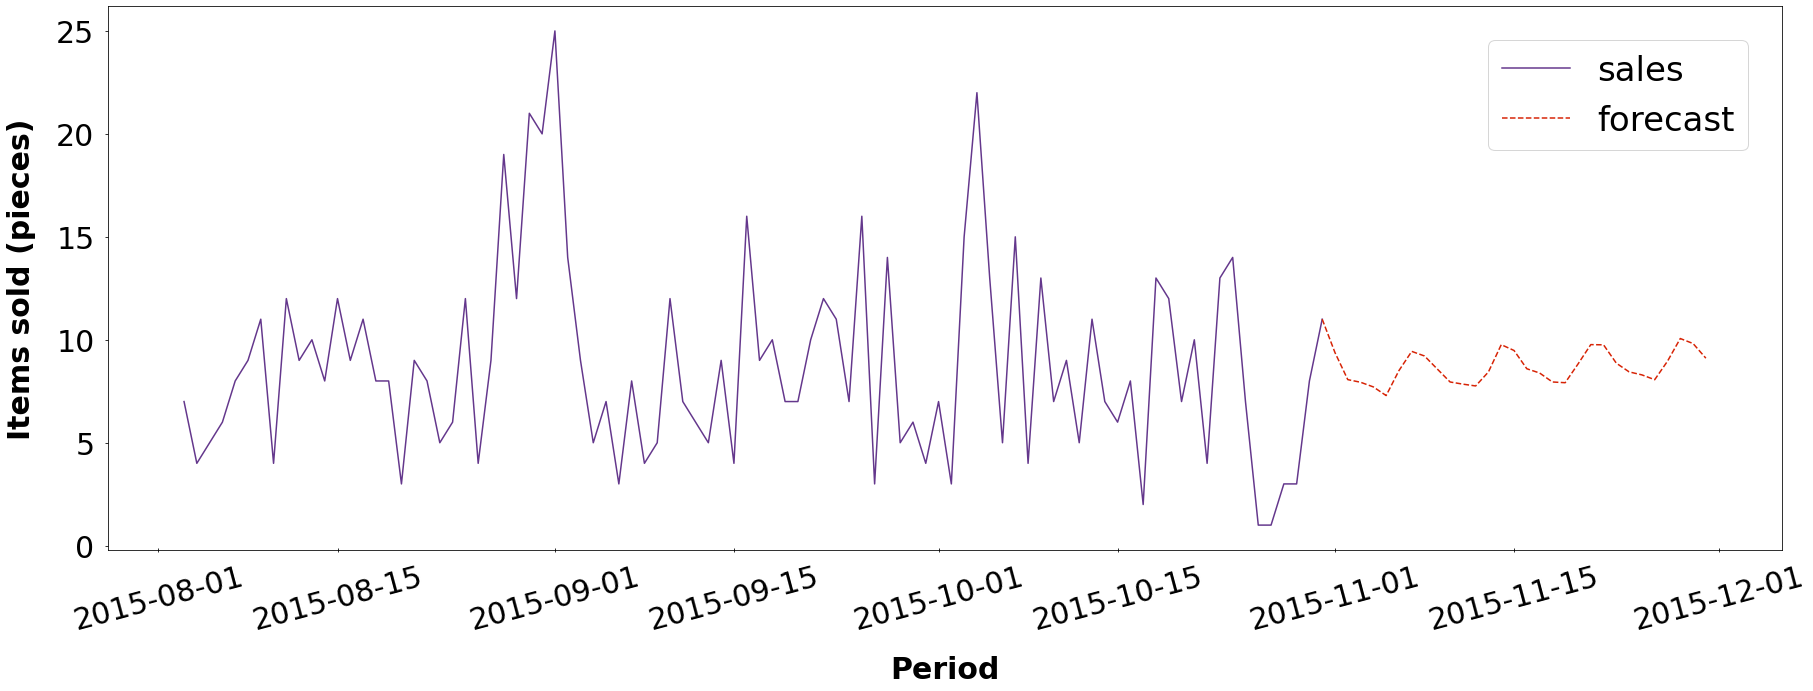
\includegraphics[width=0.9\linewidth]{external_content/graphs/final_arima_forecast.png}
  \captionsetup{justification=centering}
  \captionof{figure}{ARIMA forecast of item \texttt{5822}}
  \label{fig:arima_forecast}
\end{figure}

\vspace*{-8mm}
\begin{center}
\textit{\href{\finalARIMAurl}{The step-by-step procedure on how to finetune the \acrshort{arima} parameters can be found here.}}
\end{center}
